\chapter{Bestandssystemen}

Een computerprogramma is een verzameling instructies die toegepast
wordt op invoergegevens. Het resultaat zijn opnieuw gegevens: de uitvoer.
De gebruiker van een computersysteem wil deze gegevens vaak bewaren.
Computersystemen hebben er naast gegevensverwerking een taak bijgekregen:
gegevensopslag.

Het onderdeel van het besturingssysteem dat instaat voor de
permanente opslag van gegevens is het
\emph{bestandssysteem}. De term bestandssysteem wordt ook
soms gebruikt voor de in het systeem opgeslagen gegevens zelf. De
doelstellingen van het bestandssysteem zijn opnieuw samen te vatten als
gebruiksgemak en effici\"entie.

De gebruiker verwacht van het besturingssysteem dat het persistente
gegevensopslag aanbiedt. Het moet eenvoudig zijn om de gegevens te
organiseren en logisch te ordenen. De gegevenstoegang moet zo snel
mogelijk gaan, en er moet gestreefd worden naar een zo goed mogelijk
gebruik van de beschikbare capaciteit. Een bijkomende vereiste voor veel
systemen is het beveiligen van de gegevens, zodat b.v. verschillende
gebruikers van het systeem geen toegang hebben tot mekaars
gegevens.

\section{Fysische vs Logische gegevensordening}

\subsection{Fysische ordening: Sectoren}

Een \emph{sector} is de kleinste adresseerbare
eenheid voor gegevensopslag op een harde schijf. Een veelvoorkomende
waarde voor de sectorgrootte van een schijf is 512 bytes. Wanneer we
beschikken over een harde schijf, kunnen we dus blokjes gegevens van
512 bytes wegschrijven op een bepaald adres, en ze later terug vanop
dat adres inlezen. Hoe de gegevens over (de sectoren van) de harde
schijf verdeeld zijn noemen we de \emph{fysische
ordening} van de gegevens.

\subsection{Logische ordening: Bestanden}

De harde schijf biedt ons dus persistente gegevensopslag, maar
van gebruiksvriendelijkheid is weinig sprake. Een gebruiker wil een
\emph{logische gegevensordening}, die er b.v. voor zorgt
dat gegevens makkelijk terug te vinden zijn. In de logische ordening
wordt als basiselement meestal het bestand gebruikt. Een
\emph{bestand} is een persistent opgeslagen logische
verzameling gerelateerde gegevens.

De taak van het bestandssysteem kan omschreven worden als het
aanbieden van een gebruiksvriendelijke en logisch geordende toegang
tot de fysische opslagmedia. Het bestandssysteem vertaalt het logische
beeld van de gebruiker en de bijhorende operaties in de fysische
schijftoegangen. De gebruiker of de programma's die hij uitvoert
moeten afgeschermd worden van de complexiteit en de benodigde
boekhouding. Zo wordt een bestand altijd voorgesteld als een
aaneengesloten reeks gegevens, zelfs als dat in de fysische ordening
niet zo is. Het opzetten van de nodige gegevensstructuren voor de
fysische ordening van een bestandssysteem op een partitie noemt men
\emph{formatteren}.

\section{Bestanden}

Een bestand is een verzameling gerelateerde gegevens, die door een
gebruiker of een applicatie op een bepaalde manier ge\"interpreteerd
worden.

Opdat de gebruiker de bestanden gemakkelijk kan aanspreken krijgen
ze een naam, en opdat het bestandssysteem de gegevens kan terugvinden
moeten de adressen van de gebruikte sectoren bijgehouden worden. Het
bestandssysteem verzamelt alle gegevens over een bestand in de
\emph{bestandsbeschrijving} of \emph{file
descriptor}.

De \emph{bestandsnaam} verhoogt het gebruiksgemak
doordat de gebruiker zijn bestanden eenvoudig kan identificeren. Voor de
goede werking van het bestandssysteem is een betekenisvolle naam niet
noodzakelijk.

In ieder bestandssysteem zijn er beperkingen aan de maximale
lengte en de toegelaten karakters voor de naam. De lengte van de naam
kan beperkt zijn door de beschikbare ruimte in de bestandsbeschrijving.
Welke karakters toegelaten zijn hangt af van de gebruikte codering (b.v.
ASCII of Unicode) en het vermijden van tekens die in het systeem een
speciale betekenis hebben. Zo worden vaak de '\' of '/' gebruikt als
scheidingsteken waardoor ze niet gebruikt kunnen worden in een
bestandsnaam. Ook de hoofdlettergevoeligheid van het bestandssysteem
be\"invloedt de mogelijke bestandsnamen. Sommige systemen leggen een vaste
structuur op aan de naam. Een voorbeeld hiervan is de '8+3' structuur in
MS-DOS. De eigenlijke naam kan 8 tekens lang zijn, en wordt aangevuld
met een extensie van 3 tekens, die aangeeft welk soort gegevens het
bestand bevat.

Naast de bestandsnaam worden in de bestandsbeschrijving allerlei
andere \emph{bestandskenmerken} bijgehouden. Deze zijn
voor ieder bestandssysteem anders, maar meestal vindt men minstens de
grootte van het bestand en de tijdstippen waarop het bestand aangemaakt
en/of voor het laatst gewijzigd werd. In een besturingssysteem met
meerdere gebruikers zal ook de eigenaar van het bestandworden vermeld en
op welke manier de toegang tot het bestand wordt geregeld. Verder kan de
aard van de inhoud, de interne structuur van het bestand of een
verplichte periode van bewaring opgeslagen zijn.

Aangezien het bestandssysteem een opgegeven bestandsnaam moet
vertalen naar de plaats waar de gegevens van het bestand zich bevinden
op het extern geheugenmedium moet er ook een
\emph{plaatsaanduiding} bijgehouden worden. De manier
waarop de plaatsaanduiding wordt opgenomen in de file descriptor hangt
af van de manier waarop de fysische gegevens bewaard worden.

Om de fysische gegevenstoegang te organiseren kunnen ook extra
gegevens over de toestand van het bestand nodig zijn. Zo kan het
belanrijk zijn om te weten of het bestand in gebruik is, en of er een
kopie bestaat in het werkgeheugen of elders op de schijf.

\section{Directories}

Een computersysteem bevat tegenwoordig gemakkelijk enkele
tienduizenden bestanden. Om een overzicht mogelijk te maken in de
massale hoeveelheden aanwezige informatie is het noodzakelijk dat, net
als in een bibiotheek, een catalogus beschikbaar is. De gebruiker krijgt
vaak de mogelijkheid om deze catalogus zelf te organiseren, en kan dan
bij elkaar horende bestanden groeperen in
\emph{directories}.

Directories zijn een toevoeging aan het logische beeld dat de
gebruiker van de opgeslagen gegevens krijgt. Gelijkaardige of
gerelateerde bestanden worden nu samen aangeboden. Natuurlijk moeten de
directories ook fysisch op de schijf bijgehouden worden. Een directory
is dus ook een fysische gegevensstructuur op de schijf, die de
bestandsbeschrijvingen van de elementen (bestanden) bevat.

\section{Structuur van het bestandssysteem}

\subsection{Lineaire directory}

De meest eenvoudige organisatievorm voor een bestandssysteem is
de \emph{lineaire of vlakke directory}
(\emph{flat directory}). Hierbij worden de
bestandsbeschrijvingen van alle in het bestandssysteem aanwezige
bestanden in \'e\'en enkele directory opgenomen. Hoewel dit een erg
eenvoudige organisatievorm is, vertoont hij enkele zeer belangrijke
nadelen.

Indien het bestandssysteem een groot aantal bestanden bevat
zullen de basisbewerkingen, omwille van de grootte van de directory,
veel tijd vragen. Bovendien is een dergelijke lange lijst van
bestanden uiterst onoverzichtelijk. Tenslotte eist deze
organisatievorm dat aan elke bestand een unieke naam wordt
gegeven.

Een voordeel van dit systeem is wel dat het bij
schijvengeheugens toelaat de directory op de meest gunstige plaats van
de schijf te zetten, zodat toegang tot de informatie in de directory
zeer snel kan worden verkregen.

Omwille van de grote nadelen is het gebruik van lineaire
directories beperkt tot kleine bestandsystemen in omgevingen met
slechts \'e\'en gebruiker.

\section{Hi\"erarchisch bestandssysteem}

De meeste systemen maken gebruik van een hi\"erarchische
directorystructuur. Hierbij wordt de volledige verzameling bestanden
opgesplitst in een aantal kleinere groepen, die elk hun afzonderlijke
directory hebben. Dit laat toe bestanden met gelijkaardige
eigenschappen samen te brengen, wat de verzameling voor de gebruiker
heel wat overzichtelijker maakt.

De verschillende directories worden in een hi\"erarchisch verband
samengebracht. Een directory bevat dus bestanden en/of directories. De
directories waarnaar een directory verwijst noemen we zijn
\emph{subdirectories}.

Indien de gebruiker zorgt draagt voor een goed doordachte
groepering van de bestanden en directories zal een bestand in deze
structuur makkelijk kunnen worden teruggevonden. Bovendien is het nu
niet meer nodig dat elk bestand een unieke naam heeft: bestanden in
verschillende directories kunnen met dezelfde naam worden
aangeduid.

Toch vertoont ook deze organisatievorm nadelen. Eerst en vooral
volstaat de bestandsnaam niet meer om een bestand eenduidig aan te
wijzen. Er moet een manier worden gevonden om aan te geven waar het
bestand in de hi\"erarchische structuur te vinden is. Meestal gebruikt
men hiervoor het concept van het \emph{pad}: de
opsomming van alle directories die moeten worden doorlopen vanaf de
hoofddirectory om de directory waarin de file wordt beschreven te
bereiken.

Naast de gewone basisbewerkingen heeft de hi\"erarchische
directorystructuur ook behoefte aan bijkomende bewerkingen zoals het
toevoegen en verwijderen van directories. Om het werken in deze
structuur te vereenvoudigen wordt ook vaak een positie gedefinieerd.
De directory waarin de gebruiker zich bevindt wordt de
\emph{werkdirectory} (\emph{working
directory}) genoemd. Hierdoor moet niet telkens het
volledige pad gebruikt worden om een bestand aan te duiden. Een pad
dat vertrekt van de huidige werkdirectory wordt een
\emph{relatief pad} genoemd, een pad dat vertrekt
vanuit de wortel van de boomstructuur wordt een \emph{absoluut
pad ge}noemd. Wanneer je in een MS-DOS omgeving werkt wordt
de werkdirectory aangegeven in de commandoprompt:

\begin{verbatim}
C:\Windows\system32>
\end{verbatim}

In dit geval is de werkdirectory dus \verb|C:\Windows\system32|. Het
relatieve pad \verb|drivers\etc\hosts| verwijst vanuit deze werkdirectory
naar het bestand met absoluut pad \verb|C:\Windows\system32\drivers\etc\hosts|.

Sommige bewerkingen zullen ook heel wat complexer worden. Het
opzoeken van een bestand waarvan alleen de naam bekend is vereist nu
b.v. het recursief doorlopen van de volledige directorystructuur. Ook
het schrappen van een directory stelt een probleem: wat gebeurt er in
dat geval met de bestanden en de subdirectories waarnaar vanuit deze
directory wordt verwezen? Indien deze mee moeten worden vernietigd
moet dit eveneens op een recursieve manier gebeuren. Bovendien bestaat
daarbij het gevaar voor het onbewust schrappen van belangrijke
informatie. Daarom wordt vaak ge\"eist dat een te schrappen directory
eerst leeg wordt gemaakt.

Een hi\"erarchische directorystructuur kan verschillende vormen
aannemen: naar gelang de geldende regels spreekt men van een
boomstructuur, een algemene of een acyclische structuur.

\subsubsection{Boomstructuur}

De \emph{boomstructuur} is de eenvoudigste
hi\"erarchische structuur. Naar ieder bestand in het systeem leidt er
juist \'e\'en uniek pad, zoals in fig. \ref{boomstructuur}.

\begin{figure}
\begin{center}
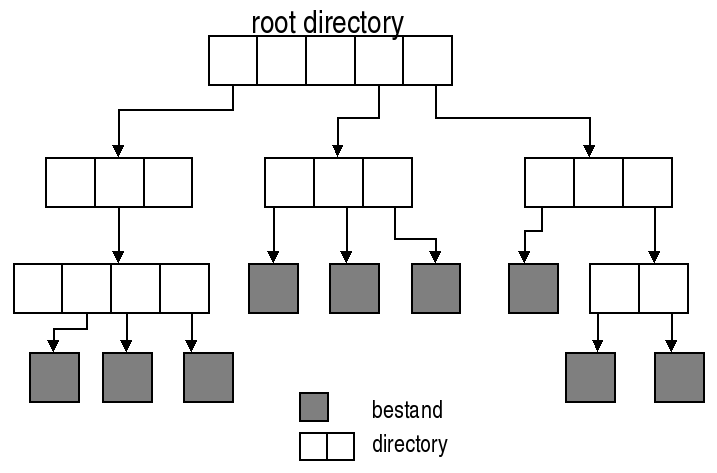
\includegraphics[width=75mm]{images/fig0401.png}
\end{center}
\caption{Boomstructuur}
\label{boomstructuur}
\end{figure}

We kunnen ook stellen dat ieder bestand vanop ieder hoger
niveau in de structuur vanuit juist \'e\'en directory bereikbaar is. We
gebruiken de term boomstructuur, omdat deze structuur zich vertakt
als een boom. In een boom is er naar ieder blad ook slechts \'e\'en
uniek pad van takken. Naar analogie met een boom wordt de directory
van waaruit de structuur vertrekt vaak wortel of \emph{root
directory} genoemd.

\subsubsection{Algemene structuur}

Wanneer we toch meer dan \'e\'en pad naar een bestand toelaten
krijgen we een \emph{algemene structuur}. Dit betekent
dat een bestand een element van twee verschillende directories kan
zijn, of dat een directory een subdirectory is van twee of meer
directories.

\begin{figure}
\begin{center}
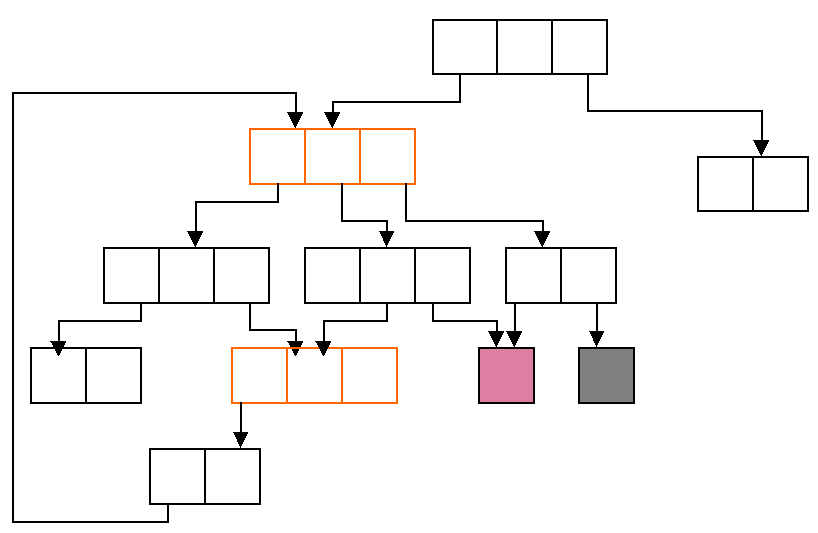
\includegraphics[width=75mm]{images/fig0402.png}
\end{center}
\caption{Algemene structuur}
\label{algstructuur}
\end{figure}

Een dergelijke veralgemening van de structuur kan handig zijn
wanneer een bestand b.v. door meerdere gebruikers wordt gebruikt, of
betrekking heeft op verschillende projecten en het dus niet
eenduidig is waar in de structuur het bestand moet bewaard
worden.

De algemene structuur laat toe dat er lussen gecre\"eerd worden
in het bestandssysteem. Dergelijke lussen veroorzaken heel wat
moeilijkheden. Iedere recursieve operatie op het bestandssysteem,
zoals b.v. het zoeken naar een bestand, zal oneindig doorgaan in
zo'n lus als het recursief algoritme niet detecteert dat het een
bepaalde directory al heeft behandeld.

Een bijkomend probleem betreft het achterblijven van
onbereikbare bestanden in het systeem na het verwijderen van een
directory. Wanneer we vertrekken van de toestand in de vorige
figuur, en we verwijderen een subdirectory van de wortel, krijgen we
de situatie in fig. \ref{problalg1}.

\begin{figure}
\begin{center}
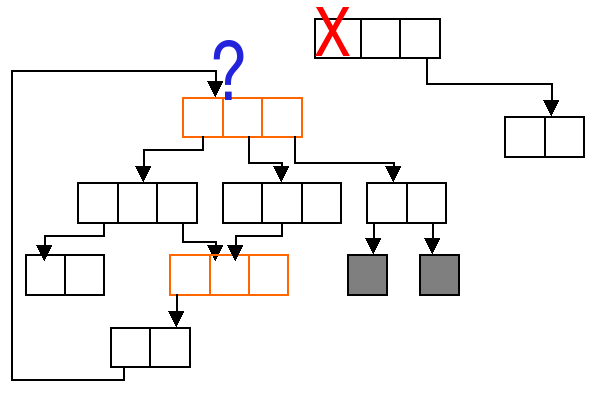
\includegraphics[width=75mm]{images/fig0403.png}
\end{center}
\caption{Problemen bij een algemene structuur}
\label{problalg1}
\end{figure}

De verwijderde subdirectory lijkt nog steeds bereikbaar, omdat
het na het verwijderen van de verwijzing vanuit de wortel nog steeds
een subdirectory is van een andere directory. Op de tekening zien we
echter in \'e\'en oogopslag dat dit geen rol speelt, omdat de directory
die nog naar de verwijderde subdirectory verwijst niet bereikbaar is
vanuit de wortel. Voor het bestandssysteem is het echter verre van
eenvoudig om een dergelijke conclusie te trekken.

Als mogelijke oplossing voor dit probleem zouden we kunnen
beslissen om altijd recursief alle subdirectories te verwijderen,
zelfs al lijken ze nog bereikbaar. Maar dan stuiten we op een tweede
probleem. Stel dat we in fig. \ref{problalg2:a} de aangeduide directory
willen verwijderen.

\begin{figure}
\centering
\begin{subfigure}{.5\textwidth}
  \centering
  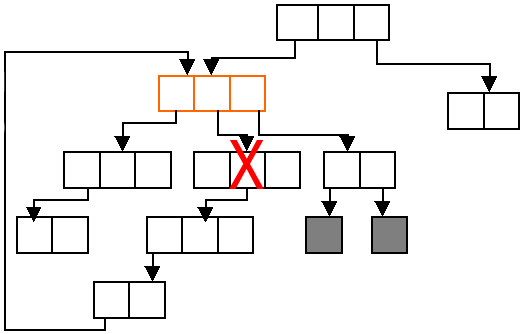
\includegraphics[width=60mm]{images/fig0404a.png}
  \caption{Voor het verwijderen}
  \label{problalg2:a}
\end{subfigure}%
\begin{subfigure}{.5\textwidth}
  \centering
  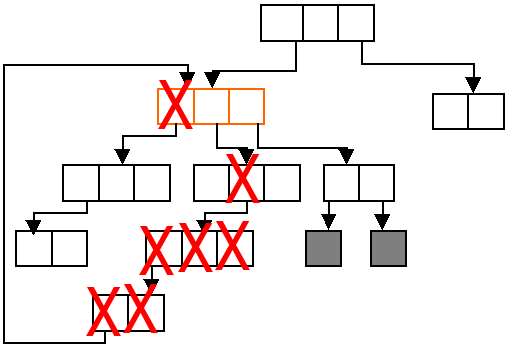
\includegraphics[width=60mm]{images/fig0404b.png}
  \caption{Na het verwijderen}
  \label{problalg2:b}
\end{subfigure}
\caption{Problemen bij een algemene structuur}
\label{problalg2}
\end{figure}


Als we dan alle onderliggende directories recursief
verwijderen, zullen we uiteindelijk een directory verwijderen die
hoger in de hi\"erarchische structuur ligt dan de directory die we
oorspronkelijk wilden verwijderen (fig. \ref{problalg2:b}). Zo zouden we ongewild grote delen
van het bestandssysteem kunnen verwijderen.

Omwille van deze problemen worden dergelijke lussen in het
bestandssysteem zelden toegelaten. Men krijgt dan een acyclische
structuur.

\subsubsection{Acyclische structuur}

De \emph{acyclische structuur} is nog steeds
algemener dan de boomstructuur, maar er mogen geen lussen voorkomen.
Het is dus een beperking van de algemene structuur om de problemen
die lussen kunnen veroorzaken te omzeilen. Lussen vermijden kan op
twee manieren.

We kunnen bij iedere operatie die een lus zou kunnen
veroorzaken een controle uitvoeren. De operatie wordt enkel
toegelaten als er geen lus ontstaat. Zo zijn we zeker dat de
structuur acyclisch zal blijven. Een groot nadeel is natuurlijk dat
de operaties op het bestandssysteem complexer en dus trager
worden.

Een eenvoudigere oplossing is het verbieden van meervoudige
verwijzingen naar directories. Wanneer enkel bestanden vanuit twee
directories kunnen benaderd worden is het onmogelijk een lus te
cre\"eren. Dit beperkt natuurlijk gedeeltelijk de mogelijkheden, maar
maakt de implementatie van een acyclische structuur
eenvoudiger.

Naast de logische structuur die aan de gebruikers
gepresenteerd wordt, moeten we ook nagaan waar de informatie wordt
weggeschreven op de schijf. We streven hierbij naar een systeem dat
de beschikbare capaciteit zo optimaal mogelijk benut, en de
schijftoegang zo snel mogelijk maakt.

\section{Aaneengesloten bestanden}

De meest voor de hand liggende manier om een bestand op de schijf
te zetten is als een aaneengesloten geheel: vanaf een bepaald adres
worden alle bytes van de file achtereenvolgens op de schijf gezet, in
een reeks op elkaar volgende sectoren. We noemen dit een
\emph{aaneengesloten bestand}.

\begin{figure}
\begin{center}
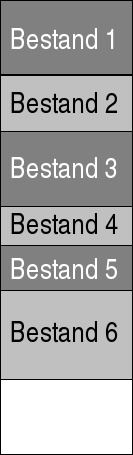
\includegraphics[width=15mm]{images/fig0405.png}
\caption{Aaneengesloten bestanden}
\end{center}
\end{figure}

Dit is een erg eenvoudige werkwijze, maar er ontstaat een
belangrijk probleem: er is een voldoende grote vrije ruimte nodig om het
bestand een plaats te kunnen geven. Zolang er geen bestanden werden
verwijderd en er nog voldoende ruimte beschikbaar is kan een nieuw
bestand gewoon achter het vorige worden geplaatst. Zo werden in het
voorbeeld 6 bestanden aangemaakt.

Naarmate het gebruik van de schijf voortduurt zal er door het
verwijderen van bestanden een steeds groter aantal afzonderlijke vrije
ruimten ontstaan. De omvang van de grootste vrije ruimte zal daarbij ook
steeds kleiner worden. Men zegt dan dat er
\emph{fragmentatie} ontstaat.

\begin{figure}
\begin{center}
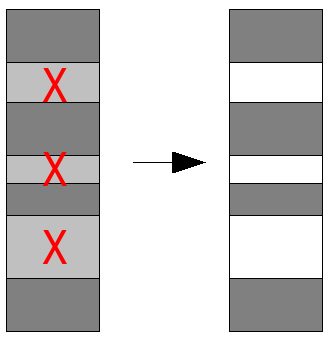
\includegraphics[width=55mm]{images/fig0406.png}
\caption{Fragmentatie}
\end{center}
\end{figure}

Wanneer een bestand toegevoegd moet worden aan een gefragmenteerd
bestandssysteem, moet er gekozen worden waar het bestand op de schijf
geplaatst moet worden. Om een geschikte locatie te kiezen moeten we in
de eerste plaats de grootte van het bestand kennen. Aangezien een
bestand kan groeien naarmate de tijd vordert, is de grootte niet gekend
op het moment dat het bestand aangemaakt wordt. De enige oplossing is om
op de een of andere manier een schatting te maken van de uiteindelijke
grootte.

Als we ervan uitgaan dat we de grootte van het bestand kennen
moeten we nog steeds beslissen in welke vrije ruimte het bestand moet
worden aangemaakt. Om deze keuze te kunnen maken houdt het
bestandssysteem een tabel bij met de adressen en de lengte van alle
vrije ruimten. Er zijn 3 algoritmes om een element van de tabel te
kiezen wanneer een nieuw bestand moet bewaard worden:

Het \emph{First Fit} algoritme kiest de eerste
vrije ruimte die voldoende groot is voor het bestand. Bij dit algoritme
is de benodigde tijd om de plaats te zoeken natuurlijk minimaal.

Wanneer men gebruik maakt van het \emph{Best Fit}
algoritme wordt de kleinste vrije ruimte gekozen die groot genoeg is
voor het bestand. \emph{Worst Fit} daarentegen kiest de
grootste beschikbare vrije ruimte. Deze algoritmes zullen trager zijn
dan first fit, omdat in dit geval de volledige tabel moet doorzocht
worden. Best and worst fit proberen de fragmentatie tegen te gaan, door
de overblijvende vrije ruimten respectievelijk zo klein of groot
mogelijk te houden.

Best fit probeert dus te vermijden dat een groter bestand dat
eventueel later aangemaakt wordt geen plaats vindt doordat een grote
vrije ruimte verkleind is. Waarschijnlijk past het bestand dat geplaatst
wordt niet helemaal, waardoor best fit vele zeer kleine vrije ruimten
cre\"eert. Worst fit probeert dit net te vermijden. Door het bestand in de
grootste vrije ruimte te plaatsen is de vrije ruimte die overblijft als
het bestand niet exact past ook zo groot mogelijk.

Het belangrijkste voordeel van het werken met aaneengesloten
bestanden is ongetwijfeld de hoge snelheid waarmee met deze bestanden
kan worden gewerkt. Door het gebruik van op elkaar volgende sectoren zal
een bestand zich meestal volledig binnen \'e\'en cylinder van de schijf
bevinden. Er gaat dan geen zoektijd verloren (door de relatief trage
armbewegingen van de schijf).

Een ander voordeel is de mogelijkheid om niet alleen sequenti\"ele,
maar ook directe toegang tot een bepaald deel van het bestand te
krijgen. Als we het startadres $s$ van het bestand, en de blokgrootte $b$
van de schijf kennen (fig. \ref{direct}) kan op eenvoudige wijze het adres $a$ worden berekend
van het blok dat de byte op positie $B$ binnen het bestand bevat\footnote{De
adressen $s$ en $a$ zijn absolute adressen, $B$ is een relatieve verwijzing
binnen het
bestand (voor $B$ beginnen we dus te tellen vanaf $s$).}:

\begin{figure}
\begin{center}
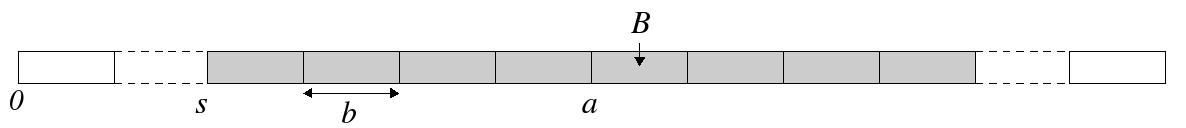
\includegraphics[width=\textwidth]{images/fig0407.png}
\end{center}
\caption{Directe toegang}
\label{direct}
\end{figure}

\begin{displaymath}
a = s + \frac{B}{b}
\end{displaymath}

Tegenover deze voordelen staan enkele ernstige nadelen. Een eerste
moeilijkheid is de verplichting een schatting te geven van de grootte
van elk nieuw bestand. Regelmatig zal bij het schrijven naar een bestand
blijken dat de voorziene ruimte niet volstaat. Dan kan het programma
worden afgebroken om later met een betere schatting te worden hernomen,
ofwel moet het bestandssysteem het programma onderbreken en het reeds
bestaande deel van het bestand naar een grotere vrije ruimte kopi\"eren.
In beide gevallen betekent dit een ernstig prestatieverlies.

Bij het gebruik van aaneengesloten bestanden zorgt fragmentatie
ervoor dat het bijna onmogelijk is de capaciteit van de schijf volledig
te gebruiken. Na een tijd kan de vrije ruimte op zo'n manier verdeeld
zijn, dat er in het totaal wel voldoende ruimte vrij is om een bepaald
bestand aan te maken, maar niet als een aaneengesloten geheel.

In dat geval is een reorganisatie van de gegevens op het schijf
nodig. zijn. Dit kan gebeuren door alle bestanden op een ander medium te
kopi\"eren, de schijf leeg te maken en er nadien alle bestanden achter
mekaar op terug te plaatsen. Zo wordt opnieuw \'e\'en grote vrije ruimte
gecre\"eerd. Dit \emph{defragmenteren} kan eventueel ook
zonder tweede medium. Bestanden worden dan verplaatst op de schijf zelf.
Het eenvoudigste algoritme om dit te doen is bovenaan beginnen, en ieder
bestand verplaatsen zodat het aansluit met het vorige. Het resultaat is
een bestandssysteem zonder fragmentatie, maar de defragmentatie is een
tijdrovend proces en dus niet erg handig.

\section{Niet-aaneengesloten bestanden}

Vasthouden aan de ruimtelijke samenhang van een bestand
bemoeilijkt het effici\"ent gebruik van de beschikbare schijvencapaciteit.
De oplossing voor dit probleem kan gevonden worden in het verdelen van
het bestand in kleinere stukken. Zo kan zelfs bij een sterk
gefragmenteerde schijf elke kleine vrije ruimte worden benut om er een
dergelijk stukje van een bestand te plaatsen.

Het gevolg is natuurlijk dat delen van eenzelfde bestand over de
schijf zullen worden verspreid. Als we met deze bestanden werken moet de
lees/schrijfkop zich vaak verplaatsen, wat erg tijdrovend is. Het
verdelen van bestanden gebeurt natuurlijk enkel wanneer er sprake is van
fragmentatie waardoor het niet meer mogelijk is het bestand
aaneengesloten te plaatsen.

Fragmentatie zal dus altijd een nadelige invloed hebben op het
gebruik van opslagmedia. Bij aaneengesloten bestanden leidt fragmentatie
tot een onvolledig gebruik van de capaciteit, en bij niet-aaneengesloten
bestanden veroorzaakt het vertraging in de bestandstoegang. In beide
gevallen is het nuttig het bestandssysteem regelmatig te
defragmenteren.

\subsection{Blokken}

De kleinst mogelijke eenheid waarin we een bestand kunnen
opsplitsen is natuurlijk een sector. Kleinere hoeveelheden gegevens
zijn niet adresseerbaar op een schijf. Vaak wordt echter een grotere
eenheid gebruikt. Het bestandssysteem groepeert een aantal sectoren in
een \emph{blok}, ook soms
\emph{cluster} genoemd. Binnen het bestandssysteem
worden de adressen van blokken gebruikt, die dan vertaald worden naar
de adressen van de juiste sectoren.

Hoe groot moeten de gebruikte blokken zijn? Een verdeling in
grotere eenheden zorgt ervoor dat het bestand in minder delen
gesplitst wordt. Hierdoor wordt het bestand minder sterk verspreid,
dus moet de leeskop van de schijf minder verplaatsingen maken. De
toegangssnelheid is dus hoger bij grotere blokken. Bovendien zal de
adresinformatie die we nodig hebben om de verschillende delen van het
bestand terug te vinden, kleiner zijn omdat het aantal delen kleiner
is.

Kleinere eenheden hebben dan weer als voordeel dat het
plaatsverlies aan \emph{interne fragmentatie} kleiner
zal zijn. Bij het verdelen van een bestand over een aantal blokken zal
het laatste blok zelden volledig gevuld zijn. Het laatste stuk van dit
laatste blok is onbruikbaar om andere gegevens op te slaan, en gaat
dus verloren. Wanneer b.v. een bestand van 5KB verdeeld wordt over
blokken van 4KB, gaat 3KB aan schijfruimte verloren. Gemiddeld zal bij
ieder bestand een half blok verloren gaan.

Bij de keuze van een blokgrootte moet dus een evenwicht gevonden
worden tussen de toegangssnelheid en het plaatsverlies. Dit is niet
eenvoudig omdat er vele factoren een rol spelen. Het verwachte aantal
bestanden en hun gemiddelde grootte bepalen b.v. mee hoe groot het
effect van de interne fragmentatie zal zijn.

Wanneer we bestanden opsplitsen moet het bestandssysteem
natuurlijk ook bijhouden waar de verschillende delen van een bestand
opgeslagen zijn. We bespreken drie manieren waarop het bestandssysteem
deze boekhouding kan bijhouden, en gaan opnieuw na wat de invloed is
op de toegangssnelheid en de plaatseffici\"entie. We mogen ook niet
vergeten te registreren welke blokken op de schijf niet in gebruik
zijn, zodat we blokken vinden wanneer b.v. een nieuw bestand moet
worden aangemaakt.

\subsection{Bestanden als gelinkte lijsten}

Een eerste mogelijkheid om niet-aaneengesloten bestanden te
beschrijven is het gebruik van gelinkte lijsten: de file descriptor
bevat het adres van het eerste blok van het bestand, en elk blok bevat
een verwijzing of pointer naar het volgende blok. Het laatste blok van
het bestand bevat een speciale pointer die aangeeft dat de lijst
stopt, soms nul-pointer genoemd.

\begin{figure}
\begin{center}
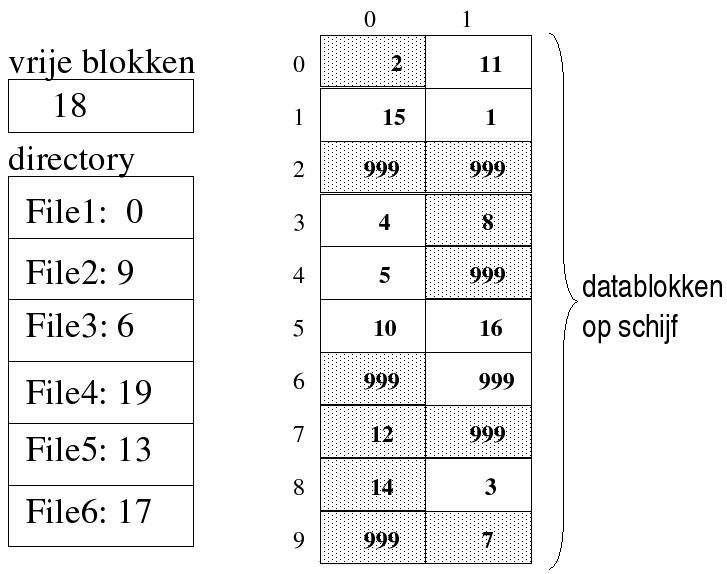
\includegraphics[width=100mm]{images/fig0408.png}
\caption{Bestanden als gelinkte lijsten van blokken}
\end{center}
\label{linklijst}
\end{figure}

Het voorbeeld in fig. \ref{linklijst} bevat een directory zes bestanden. Bij ieder
bestand wordt het adres van het eerste blok bijgehouden. In dat blok
staat het adres van het volgende blok, ofwel '999' dat de nul-pointer
voorstelt.

De blokken waarover File5 verspreid is zijn dus: 13, 8 en
14.

De vrije blokken worden ook d.m.v. een gelinkte lijst
bijgehouden. Ieder vrij blok bevat het adres van het volgende vrije
blok.

Het belangrijkste voordeel van deze methode is dat de
adresinformatie weinig plaats inneemt. In een bestandsbeschrijving
moet maar \'e\'en adres bijgehouden worden, dat van het eerste blok. Dit
zorgt ervoor dat de bestandsbeschrijvingen klein blijven. Ze zijn ook
allemaal even groot, onafhankelijk van de grootte van het
bestand.

Het grootste bezwaar tegen het werken met gelinkte lijsten is
ongetwijfeld de vaststelling dat directe toegang hier niet mogelijk
is. De enige manier om bij een bepaald deel van een bestand te komen
is immers de ketting van verwijzingen te volgen tot bij de gezochte
plaats. Daartoe moeten alle voorafgaande blokken \'e\'en na \'e\'en worden
ingelezen, zodat er eigenlijk sprake is van sequenti\"ele toegang.
Bovendien kunnen de opeenvolgende blokken sterk verspreid zijn over de
schijf, waardoor de toegangssnelheid erg laag kan liggen.

\begin{figure}
\begin{center}
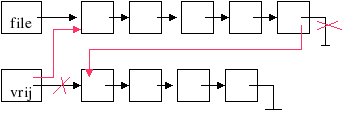
\includegraphics[width=70mm]{images/fig0409.png}
\end{center}
\caption{Gelinkte lijst met verwijzing naar lege blokken}
\label{linklijsteff}
\end{figure}

We kunnen de structuur effici\"enter maken door enkele
aanpassingen, zoals aangegeven in fig. \ref{linklijsteff}. Het verwijderen van een bestand verloopt erg traag omdat
de ketting van alle blokken doorlopen moet worden om de nul-pointer te
vervangen door een verwijzing naar het eerste blok van de lijst met
vrije blokken\footnote{Omgekeerd zou ook kunnen, we zouden de nul-pointer in het
laatste blok uit de lijst van vrije blokken kunnen vervangen door een verwijzing
naar het eerste blok van het verwijderde bestand. In het algemeen zal de
hoeveelheid vrije ruimte echter groter zijn dan het te verwijderen bestand,
waardoor het op die manier nog trager zou gaan.}

Door in de bestandsbeschrijving ook een pointer naar het laatste
blok bij te houden kunnen we het verwijderen van een bestand
versnellen.

Wanneer er iets misloopt met een verwijzing gaat een deel van
een bestand verloren, of kan een bestand soms onterecht verwijzen naar
een deel van een ander bestand. Wanneer het beschadigde bestand
verwijderd wordt gaat ook een deel van dit andere bestand verloren.
Het is ook mogelijk dat er schijfruimte verloren gaat als er iets
misloopt met de lijst met vrije blokken.

Om dergelijke problemen op te vangen wordt soms gewerkt met een
\emph{dubbel gelinkte lijst}, waarin ieder blok ook
verwijst naar het vorige blok in de lijst (zie fig. \ref{dubellink}). Een foutieve verwijzing kan
dan hersteld worden door de lijst van achter naar voor te
doorlopen.

\begin{figure}
\begin{center}
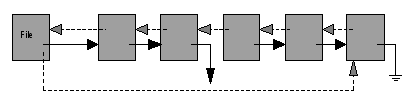
\includegraphics[width=90mm]{images/fig0410.png}
\caption{Dubbel gelinkte lijst}
\label{dubellink}
\end{center}
\end{figure}


\subsection{Bestanden met indexblokken}

De onmogelijkheid tot directe toegang bij een gelinkte lijst van
blokken wordt veroorzaakt door de verspreiding van de adresinformatie
doorheen het bestand. Dit probleem kan worden opgelost door de
adressen van de verschillende onderdelen van een bestand te verzamelen
in een speciaal daarvoor voorbehouden blok op schijf: een
\emph{indexblok}. In de file descriptor zal dan als
plaatsaanduiding het adres van dit indexblok worden opgenomen.

\begin{figure}
\begin{center}
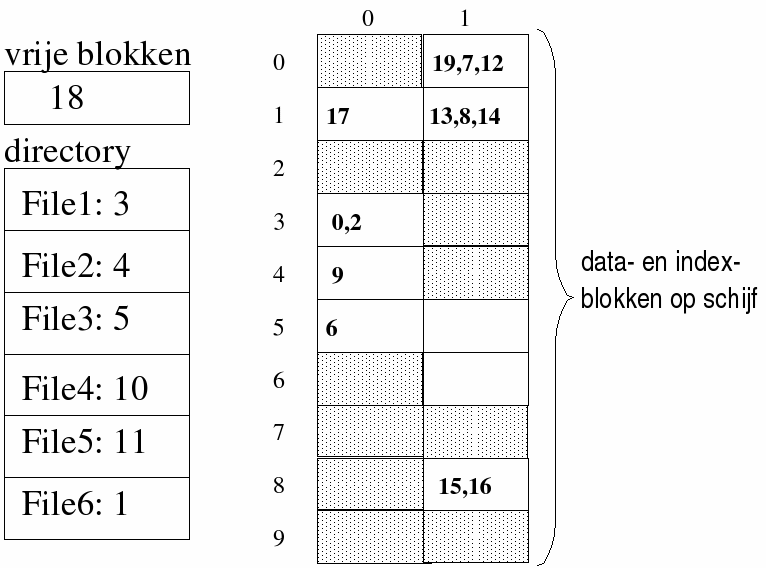
\includegraphics[width=120mm]{images/fig0411.png}
\caption{Bestanden met indexblokken}
\label{indexblokken}
\end{center}
\end{figure}

In fig. \ref{indexblokken} bevat iedere bestandsbeschrijving in de
directory het adres van een indexblok. De indexblokken zijn dus 3, 4,
5, 10, 11 en 1.

Elk van deze indexblokken bevat de adressen van de blokken met
de eigenlijke gegevens van het bestand.

Ook de vrije blokken worden bijgehouden in een indexblok
(18).

Indien \'e\'en blok niet volstaat om alle adresinformatie op te
slaan zijn er verschillende oplossingen. Men kan een gelinkte lijst
van indexblokken cre\"eren, of men kan een \emph{hi\"erarchische
index-structuur} opbouwen. Hierbij verwijst het eerste
indexblok niet naar delen van het bestand, maar naar indexblokken die
de adressen van de blokken met gegevens bevatten. Men kan een
dergelijke hi\"erarchische structuur zo diep maken als men wil.

Het grootste voordeel van een structuur met indexblokken is de
toegangssnelheid. Wanneer een bestand geopend wordt kan het indexblok
volledig in het geheugen geladen worden. Hierdoor is directe toegang
mogelijk, in tegenstelling tot de structuur met gelinkte lijsten.
Zelfs bij seri\"ele toegang is er een kleine snelheidswinst, omdat er
niet moet gewacht worden tot het bestandssysteem het adres van het
volgende blok uit het vorige blok gelezen heeft kunnen er meerdere
leesopdrachten tegelijk aan de schijf doorgegeven worden.

Een nadeel van indexblokken is dat ze schijfruimte innemen. Het
gegeven voorbeeld voor gelinkte lijsten en indexblokken is hetzelfde,
maar in het eerste geval hadden we 9 vrije blokken over en bij
indexblokken zijn er dat maar 2. Dit komt omdat er per bestand \'e\'en
blok extra nodig is: het indexblok.

Dit plaatsverlies is vooral groot wanneer er veel kleine
bestanden voorkomen in het systeem. Wanneer een bestand maar \'e\'en blok
groot is neemt het 2 keer zoveel plaats in op de schijf door het
indexblok. Hoe groter het bestand, hoe kleiner het relatieve verlies.
Op een bestand van 100 blokken is \'e\'en indexblok een minder groot
verlies.

Daarom wordt in de bestandsbeschrijving vaak plaats voorzien
voor een klein aantal adressen van blokken van het bestand. Als de
hoeveelheid benodigde blokken onder dit aantal blijft, moet er geen
indexblok gebruikt worden. De toegang tot deze kleine bestanden is dan
ook iets sneller omdat er \'e\'en schijftoegang uitgespaard wordt.

De toegangssnelheid kan verder worden geoptimaliseerd door
zogenaamde extents te gebruiken in plaats van afzonderlijke blokken.
Een \emph{extent} is een verzameling opeenvolgende
blokken op de schijf (fig. \ref{extents}). Hierdoor zullen grotere delen van een file op
een zelfde plaats van de schijf terechtkomen, zodat het lezen of
schrijven minder onderbroken hoeft te worden voor een verplaatsing van
de leeskop. Indien de extents gemiddeld voldoende groot zijn zal ook
minder informatie moeten worden opgeslagen in de indexblok. Het adres
van het eerste blok en de lengte van de extent zijn voldoende. In de
figuur verwijst indexblok 3 naar 2 extents.

\begin{figure}
\begin{center}
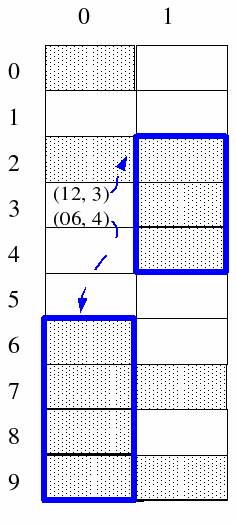
\includegraphics[width=35mm]{images/fig0412.png}
\caption{Extents}
\label{extents}
\end{center}
\end{figure}


\subsection{Bestanden beschrijven in een file map}

In de derde oplossing beschrijven we de inhoud van de schijf in
een aparte tabel. In deze tabel, de \emph{file map},
wordt voor ieder blok van de schijf aangegeven of het vrij is, en
indien niet, tot welk bestand het behoort.

De eenvoudigste versie van een file map is een bitvector, die
voor ieder blok aangeeft of het vrij is of niet. Met ieder blok komt
een bit overeen, 1 betekent dat het blok in gebruik is, 0 betekent dat
het blok beschikbaar is. Deze structuur zou kunnen gebruikt worden
i.p.v. een gelinkte lijst of indexblokken met vrije blokken.
Vergeleken met indexblokken zorgt zo'n bitvector van vrije blokken
voor minder plaatsverlies. De vaste lengte van de bitvector (1 bit per
blok) is wel nadelig als er weinig vrije blokken zijn. Als er een vrij
blok is ziet de bitvector er namelijk als volgt uit:
111...1110111...111.

Met elk blok (of andere eenheid) komt een element van de tabel
overeen. Een vrij blok wordt aangeduid door een speciale code. De
elementen, behorend bij de blokken die samen een bestand vormen,
bevatten pointers zodat ze een gelinkte lijst vormen. Het laatste
element in de lijst bevat een code om het einde van het bestand aan te
geven. De plaatsaanduiding in de file descriptor bestaat uit de index
van het element dat overeenstemt met het eerste blok in de
file.

\begin{figure}
\begin{center}
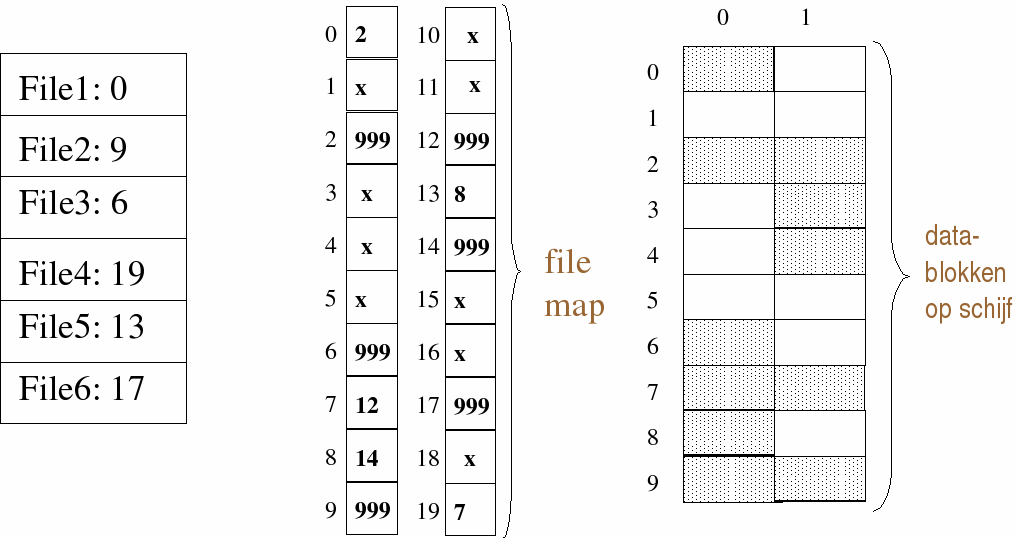
\includegraphics[width=\textwidth]{images/fig0413.png}
\caption{File map}
\label{filemap}
\end{center}
\end{figure}

In fig. \ref{filemap} wordt opnieuw hetzelfde voorbeeld als bij de twee vorige
structuren getoond. De file descriptor van File5 verwijst nu naar het element
op positie 13 in de file map. Dit leert ons dat het blok op adres 13
het eerste blok van het bestand File5 is, en op positie 13 in de file
map vinden we de index van het volgende blok. Blokken 8 en 14
vervolledigen dus het bestand.

Een groot voordeel van een file map is de mogelijkheid om de
volledige beschrijving van een schijf in het centrale geheugen te
brengen. Dit maakt directe toegang tot de bestanden mogelijk en
bespaart ook telkens het afzonderlijk inlezen van adresinformatie. We
werken eigenlijk weer met een gelinkte lijst, maar nu is de volledige
lijst van adressen al beschikbaar in het werkgeheugen.

Men kan er ook op een eenvoudige wijze voor zorgen dat een
bestand zo goed mogelijk gegroepeerd blijft: de combinatie van de
beschrijving van de met de adresgegevens van het bestand in \'e\'en tabel
laat toe bijkomende ruimte voor het bestand te zoeken in de
onmiddellijke nabijheid van het laatst toegekende blok.

\section{Directories (2)}

Nu we de fysische opslag van bestanden op de schijf bekeken
hebben, keren we nog even terug naar de directories. We weten dat er
verschillende logische structuren zijn, zoals de cyclische en acyclische
hi\"erarchie\"en. Maar ook deze directories moeten ergens op de schijf een
plaats krijgen.

Een directory is een verzameling bestandsbeschrijvingen. Er zijn
verschillende fysische structuren mogelijk om deze
bestandsbeschrijvingen op een schijf op te slaan: een gewone tabel, een
gesorteerde tabel, een hashtabel of een gelinkte lijst. Om een keuze te
kunnen maken beschouwen we vooral de snelheid waarmee bewerkingen in de
directory kunnen worden uitgevoerd. Deze basisbewerkingen zijn het
opzoeken, toevoegen en verwijderen\footnote{Merk op dat het verwijderen van een
bestandsbeschrijving uit een directory veronderstelt dat we de
bestandsbeschrijving eerst zoeken.} van een bestandsbeschrijving uit de
directory.

\subsection{Tabel}

Wanneer we de bestandsbeschrijvingen in een tabel bijhouden, zal
vooral het opzoeken van een bestandsbeschrijving relatief veel tijd
vragen. We moeten de tabel doorlopen tot we het gezochte element
vinden. In het beste geval is het het eerste element, in het slechtste
geval het laatste. Gemiddeld zullen we de halve tabel moeten
doorzoeken.

Het toevoegen van een file descriptor kan zeer snel gebeuren,
aangezien die gewoon achteraan kan bijgeplaatst worden.

\subsection{Gesorteerde tabel}

Om het opzoeken in een tabel te versnellen kan de tabel
gesorteerd worden. Het is dan mogelijk om het binair zoeken toe te
passen: bekijk het middelste element, en dan weet je of het gezochte
element ervoor of erachter ligt. Zo kan je onmiddellijk de helft van
de tabel negeren, en op dezelfde manier verderzoeken in de
overgebleven helft.

Wanneer de 1000 elementen van een tabel niet gesorteerd zijn
moeten we gemiddeld 500 elementen bekijken vooraleer we het gezochte
element vinden. Bij binair zoeken in een gesorteerde tabel met 1000
elementen vinden we wat we zoeken na het bekijken van slechts 10
elementen\footnote{Je kan dit als volgt berekenen: Aangezien telkens de helft
van de elementen wegvallen hebben we er na het bekijken van 1 element nog 500
over. Na nog een element te bekijken zijn het er nog 250. De reeks is dus: 1000,
500, 250, 125, 63, 32, 16, 8, 4, 2, 1. Na 10 stappen blijft er slechts \'e\'en
element over. Wiskundig gezien berekenen we log2(1000), wat ongeveer gelijk is
aan 9,97.}. Wanneer we een tabel met 1.000.000 elementen binair doorzoeken zijn
20 stappen voldoende, terwijl we gemiddeld er 500.000 elementen zouden moeten
bekijken als de tabel niet gesorteerd zou zijn.

Doordat we de tabel gesorteerd moeten houden zal het toevoegen
van file descriptors natuurlijk wel trager verlopen. We moeten immers
eerst de juiste plaats zoeken. Dit zoeken kan ook binair, maar dan
moeten alle achterliggende elementen nog opgeschoven worden om plaats
te maken voor de nieuwe bestandsbeschrijving. Bij het verwijderen
moeten we de legen plaats opvullen door alle volgende elementen een
plaats naar voor te schuiven.

\subsection{Hashtabel}

Een hashtabel is een structuur die zeer effici\"ent opzoeken
toelaat. De positie in de tabel wordt berekend met behulp van de
hash-functie. In dit geval zal de gekozen hash-functie de bestandsnaam
transformeren in een geheel getal. De bestandsbeschrijving zal dan op
deze positie in de hashtabel bewaard worden. Wanneer we een
bestandsbeschrijving zoeken, berekenen we de hashwaarde van de
bestandsnaam, en we kennen onmiddellijk de positie waarop de gezochte
file descriptor staat.

Een mogelijk probleem zijn \emph{collisions} of
\emph{botsingen}. Wanneer de hash-functie voor twee
verschillende bestandsnamen dezelfde positie teruggeeft spreken we van
een botsing. Dan worden op die plaats in de tabel meestal
verschillende elementen bijgehouden, en moet in deze verzameling
elementen op een klassieke manier gezocht worden. Hoe groter de
hashtabel (dus hoe meer posities, en hoe meer mogelijke uitkomsten
voor de hash-functie), hoe kleiner de kans op een botsing. Het nadeel
is natuurlijk dat er meer plaats verloren gaat voor de grotere
tabel.

In gunstige omstandigheden levert de hash-functie dus
onmiddellijk de plaats van een op te zoeken file descriptor. Ook het
toevoegen of verwijderen van file descriptors kan zeer snel
gebeuren.

\subsection{Gelinkte lijst}

Ook een directory kan bijgehouden worden als een gelinkte lijst.
In de tabel verwijst ieder element naar de positie van het volgende.
We moeten dan alleen de startpositie kennen.

\begin{figure}
\begin{center}
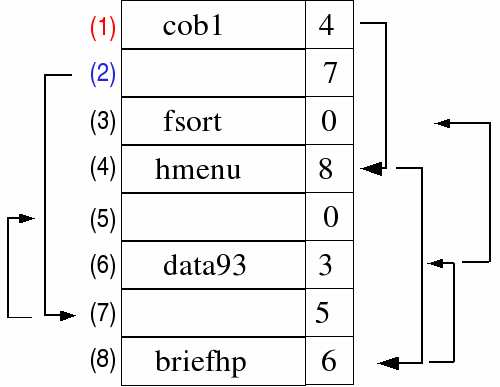
\includegraphics[width=60mm]{images/fig0414.png}
\caption{Directory als gelinkte lijst}
\label{dirlinklijst}
\end{center}
\end{figure}


In fig. \ref{dirlinklijst} is (1) de startpositie voor de directory. (2) is het begin van de lijst met vrije plaatsen in de tabel. Een verwijzing naar 0 geeft het einde van de lijst aan.

Wat betreft het opzoeken van een element in de lijst is deze
structuur te vergelijken met de klassieke tabel. Het moet sequentieel
gebeuren. Zelfs als de elementen van de lijst gesorteerd zouden zijn
is binair zoeken niet zoveel effici\"enter, aangezien we geen
rechtstreekse toegang hebben tot het middelste element.

Bij het toevoegen en verwijderen daarentegen vermijden we het
verschuiven van de achterliggende elementen op plaats te maken of om
een vrijgekomen plaats op te vullen. We kunnen gewoon de verwijzingen
aanpassen, en alle elementen kunnen op hun plaats blijven staan. Het
geringe plaatsverlies door de verwijzing naar de volgende
bestandsbeschrijving levert dus snelheidswinst bij deze
operaties.

\section{Voorbeeld 1: FAT}

Het FAT-bestandssysteem is het oorspronkelijke bestandssysteem van
het MS-DOS besturingssysteem. Voor steeds groter wordende harde schijven
raadt Microsoft vanaf Windows NT het NTFS bestandssysteem aan, maar FAT
wordt nog steeds gebruikt op diskettes en allerlei USB-opslagmedia zoals
MP3-spelers en digitale camera's.

\subsection{File Allocation Table}

\emph{FAT} staat voor \emph{File Allocation
Table}. Deze FAT is een file map met daarin de nodige
informatie over ieder blok van de schijf. Een FAT-partitie bevat een
boot sector, 2 kopie\"en van de FAT, en een datagebied dat de
directories en bestanden bevat.

In de FAT wordt voor ieder blok van de schijf \'e\'en van vijf
mogelijkheden bijgehouden. Wanneer het blok een onderdeel van een
bestand is bevat het overeenkomstige FAT-element het adres van het
volgende blok van het bestand, zoals hierboven algemeen beschreven
voor file maps. Het laatste blok van een bestand wordt aangeduid met
de End Of File (EOF)-code 0xFFFF, en een vrij blok met 0x0000. Er zijn
ook codes om gereserveerde en slechte blokken.

Er zijn verschillende varianten van het FAT bestandssysteem. De
oorspronkelijke versie wordt nu FAT12 genoemd, naast de nieuwere
versies FAT16 en FAT32. Het getal in de naam van deze systemen duidt
aan hoeveel bits er gebruikt worden voor ieder element in de FAT. In
een FAT12 systeem bevat ieder element van de FAT dus 12 bits.

Het aantal bits dat een FAT-element bevat bepaalt welke adressen
gebruikt kunnen worden voor de blokken. In een FAT12 tabel zijn er
voor ieder element $2^{12}$ of $4096$
mogelijkheden. Dat betekent dat er maximum 4096 verschillende adressen
kunnen gebruikt worden. Wanneer de blokgrootte 512 B (1 sector) is,
betekent dit dat er niet meer dan 4096 x 512 B of 2MB kunnen
geadresseerd worden. Omwille van deze limiet op de schijfgrootte was
het nodig om de nieuwe versies FAT16 en FAT32 in te voeren. Met
dezelfde blokgrootte kan een FAT32 systeem een schijf van 2 terabyte
adresseren. We stellen dus vast dat de maximale adresseerbare
schijfcapaciteit bepaald wordt door het beschikbaar aantal bits voor
het adres, maar dat ook de blokgrootte een rol speelt. Hoe groter de
blokken, hoe groter de maximale capaciteit.

De totale grootte van de FAT-tabel speelt ook een belangrijke
rol, aangezien we omwille van de performantie de volledige tabel in
het werkgeheugen willen houden. Aangezien bij een FAT12
bestandssysteem $2^{12}$ of $4096$ verschillende
adressen mogelijk zijn, is dit ook het maximaal aantal elementen in de
tabel (1 element per blok). De grootte van de tabel is dan
$2^{12}x12$ bits, dus $49152$ bits of 6 KB. Voor
FAT32 wordt dit $2^{32}x32$ bits, wat
overeenkomt met 16 GB. Het is duidelijk niet haalbaar om een
dergelijke tabel in het werkgeheugen bij te houden.

Door de blokgrootte te verhogen kunnen we dus ofwel zorgen voor
een grotere adresseerbare schijfcapaciteit, of voor een kleinere
FAT-tabel. De volgende tabel geeft de standaard blokgrootte voor
FAT-bestandssystemen in Windows XP:

\begin{center}
\begin{tabular}{|l|l|}
\hline
Partitiegrootte  & Blokgrootte \\
\hline
33MB - 64MB      & 512B \\
65MB - 128MB     & 1KB \\
129MB - 256MB    & 2KB \\
257MB - 8GB      & 4KB \\
8GB - 16GB       & 8KB \\
16GB - 32GB      & 16KB \\
$>$ 33GB         & Niet ondersteund\\
\hline
\end{tabular}
\end{center}

Wanneer je dus een partitie van 12 GB als FAT32 formatteert in
Windows XP, zullen er blokken van 8 KB gebruikt worden. Dit betekent
dat ieder blok 16 sectoren op de schijf inneemt. Merk op dat je voor
partities van meer dan 32 GB het NTFS bestandssysteem moet gebruiken
in Windows XP.

\subsection{Directories}

De logische structuur van het FAT bestandssysteem is een
boomstructuur. Fysisch wordt een directory voorgesteld als een gewone
tabel. Deze tabel wordt op dezelfde manier opgeslagen op de schijf als
een gewoon bestand: de blokken waarop de directory-tabel staan worden
via een gelinkte lijst in de FAT bijgehouden.

In FAT12 en FAT16 staat de root-directory onmiddellijk na de 2
kopie\"en van de FAT. In FAT32 is dit niet meer verplicht. In de
directory-tabel neemt iedere bestandsbeschrijving 32 bytes in. De
betekenis van deze 32 bytes wordt hieronder aangegeven.

\begin{center}
\begin{tabular}{|l|l|l|}
\hline
Veld                              & Positie & Lengte \\
\hline
Naam                              & 0       & 8      \\
Extensie                          & 8       & 3      \\
Attributen                        & 11      & 1      \\
Tijdstip Creatie                  & 12      & 1      \\
Hoogste bytes startadres          & 20      & 2      \\
Startadres (FAT32: laagste bytes) & 26      & 2      \\
Grootte                           & 28      & 4      \\
\hline
\end{tabular}
\end{center}

We zien hier onmiddellijk waarom bestandsnamen in MS-DOS beperkt
zijn tot 8 karakters voor de naam en 3 karakters voor een
extensie.

Het attributen-veld verdient nog wat aandacht. Elk van de 8 bits
komt over\'e\'en met een bepaald attribuut, en duidt aan of dit attribuut
op het element van de directory van toepassing is. E\'en van de
attributen is het 'directory' attribuut. Als hier een '1' staat
beschijft dit element een subdirectory, anders een bestand. Voor ieder
bestand zijn er de read-only, hidden, system en archive
attributen.

\begin{figure}
\begin{center}
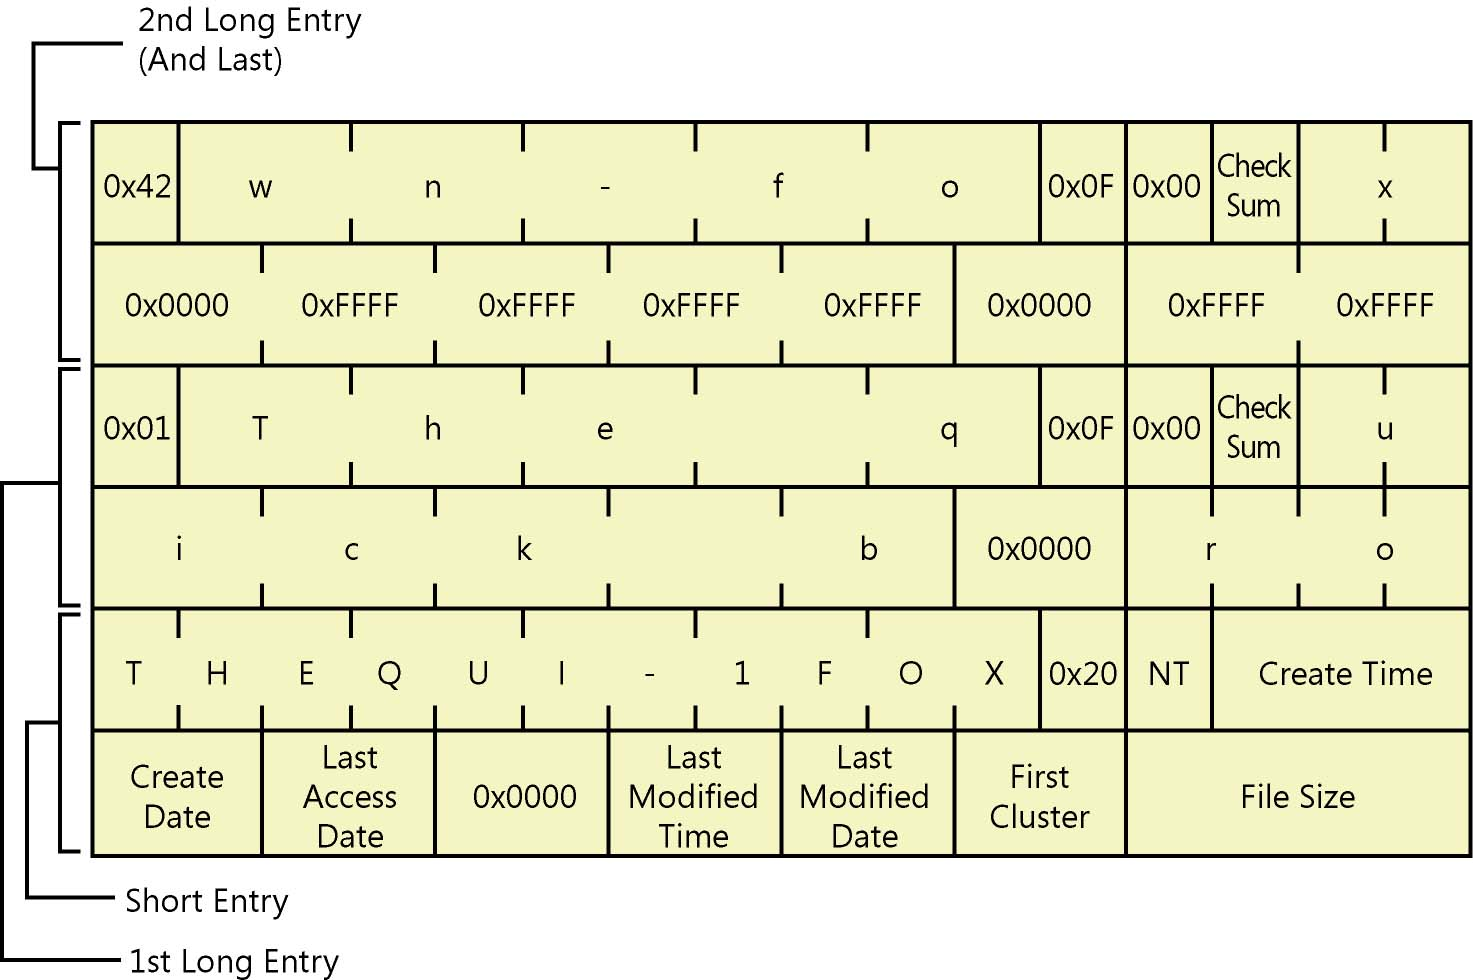
\includegraphics[width=\textwidth]{images/fig0415.jpg}
\caption{Lange bestandsnamen in FAT \tiny{afbeelding uit ``Windows XP Professional Resource Kit''}}
\label{fatlangnaam}
\end{center}
\end{figure}


Het Volume Label attribuut wordt normaal slechts voor \'e\'en
speciaal element van de root directory gebruikt. In iedere andere
context negeert MS-DOS dit bestanden waarbij dit attribuut op '1'
staat. Hiervan is handig gebruik gemaakt om in Windows de mogelijkheid
te voorzien om langere bestandsnamen te gebruiken in
FAT-bestandssystemen (zie fig. \ref{fatlangnaam}).

De lange naam wordt verspreid over bepaalde delen van meerdere
tabelelementen. Het volume-attribuut van deze elementen wordt op 1
gezet, zodat MS-DOS ze negeert. MS-DOS gebruikt nog steeds een
verkorte versie van de naam die in de eigenlijke bestandsbeschrijving
bijgehouden wordt.

\section{Voorbeeld 2: NTFS}

NTFS staat voor New Technology File System. Het is het standaard
bestandssysteem voor Windows NT, 2000, XP en 2003 Server. Het lost
enkele problemen met FAT op en bevat heel wat extra
functionaliteit.

NTFS bestandsnamen kunnen 255 tekens lang zijn, en de tekens
worden m.b.v. unicode bewaard. Hierdoor kunnen naast het gewone Westerse
alfabet allerlei andere tekens gebruikt worden.

\subsection{Master File Table}

NTFS maakt gebruik van een \emph{Master File
Table} (\emph{MFT}). In deze tabel wordt
voor ieder bestand 1 bestandsbeschrijving bijgehouden. Deze
beschrijving bevat naast de bestandsnaam, de grootte en de
toegangsdata informatie over de toegangsrechten tot het
bestand.

In tegenstelling tot de File Allocation Table in het FAT-systeem
is de MFT dus geen file map. De MFT bevat \'e\'en record per bestand, en
niet \'e\'en record per blok op de schijf. Hierdoor is de grootte van de
MFT variabel. Standaard wordt 12,5\% van de partitie voorzien voor de
MFT, en de overige 87,5\% is beschikbaar voor gegevens. Wanneer het
datagebied echter vol is, en de MFT neemt niet de voorzien 12,5\% van
de partitie in kan die ook voor data gebruikt worden.

\begin{figure}
\begin{center}
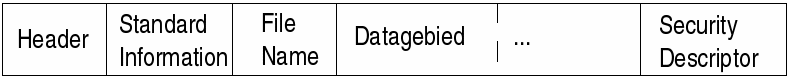
\includegraphics[width=100mm]{images/fig0416.png}
\caption{MFT-record}
\label{mftrecord}
\end{center}
\end{figure}

Een record in de MFT bevat attributen. In fig. \ref{mftrecord} worden de
attributen getoond die voor ieder bestand aanwezig zijn. Welke overige attributen
gebruikt worden staat niet vast in de specificatie van NTFS. De
gebruikte attributen op de partitie worden in het systeembestand
\$AttrDef bijgehouden.

De standaardinformatie omvat de grootte van het bestand, de
toegangsdatums en andere eigenschappen. De toegangsrechten worden
bewaard in de security descriptor. Omdat attributen geen vaste lengte
hebben is er een hoofding nodig die de structuur van het record
beschrijft.

Wanneer de inhoud van een attribuut te groot wordt om in het
MFT-record te bewaren wordt het attribuut non-resident gemaakt. Dit
betekent dat de inhoud van het attribuut in vrije blokken in het
datagebied bewaard wordt, en dat het MFT-record een verwijzing naar
deze blokken bevat.

\begin{figure}
\begin{center}
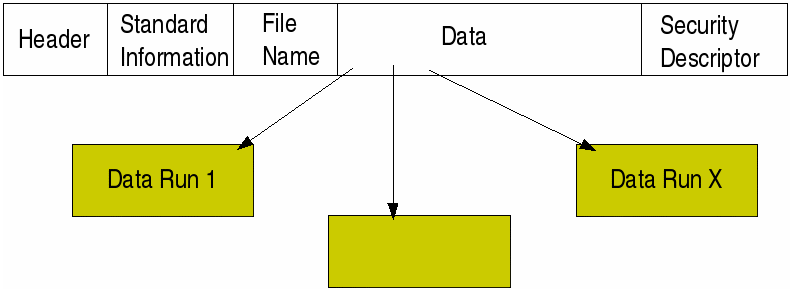
\includegraphics[width=100mm]{images/fig0417.png}
\caption{Data Runs}
\label{dataruns}
\end{center}
\end{figure}

Het data-attribuut in een MFT-record bevat verwijzingen naar
blokken in het datagebied. We kunnen het data-attribuut dus beschouwen
als een indexblok. Om de toegangssnelheid te verhogen en de
hoeveelheid adresinformatie te beperken wordt gebruik gemaakt van
extents, die in de context van NTFS vaak data runs of streams genoemd
worden (fig. \ref{dataruns}).

Voor kleine bestanden wordt de inhoud van het bestand zelf
binnen het data-attribuut in het MFT-record opgeslagen. Dit zorgt
ervoor dat met dergelijke bestanden zeer snel gewerkt kan worden. Zo
gauw het bestand is opgezocht is directe toegang mogelijk zonder
verdere schijftoegangen. Dit gebeurt typisch voor bestanden die
kleiner zijn dan 1 tot 1,5 KB. Als we dit geval als standaard
beschouwen, kunnen we zeggen dat als een bestand te groot wordt het
data-attribuut non-resident gemaakt wordt.

Wanneer een bestand zo groot wordt dat de verschillende data
runs niet meer binnen het data-attribuut kunnen beschreven worden is
het mogelijk om het data-attribuut zelf buiten het MFT-record op te
slaan (fig. \ref{nonresdata}). Deze structuur kan nog verder uitgebreid worden zodat de ruimte
van het data-attribuut in de MFT-record een indirect indexblok
wordt.

\begin{figure}
\begin{center}
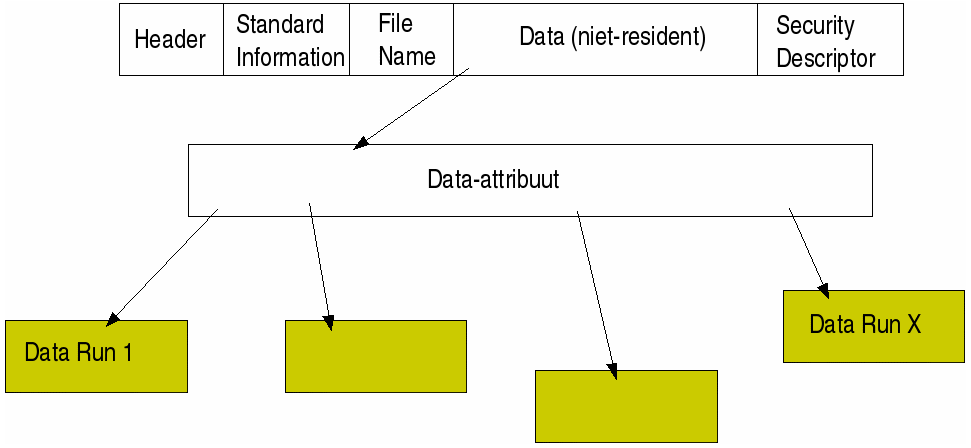
\includegraphics[width=120mm]{images/fig0418.png}
\caption{Niet-resident data-attribuut}
\label{nonresdata}
\end{center}
\end{figure}

Door deze flexibele structuur is er bij NTFS geen sprake van een
maximale bestandsgrootte. In theorie kan \'e\'en bestand de beschikbare
capaciteit van de volledige partitie innemen.

\subsection{Directories}

De logische structuur van NTFS is een boomstructuur, net als bij
FAT. Voor directories wordt ook een record in de MFT aangemaakt. Een
directory-record heeft extra attributen die verwijzingen bevatten naar
de bestanden en subdirectories. Net als bij gewone bestanden worden
deze gegevens voor een kleine directory in het record
bijgehouden.

De fysische structuur van de inhoud van een directory wordt
bijgehouden m.b.v. B-bomen. Dit zijn vrij ingewikkelde gebalanceerde
en gesorteerde boomvormige gegevensstructuren die snel opzoeken en
toevoegen van elementen toelaten.

\section{Second Extended Filesystem}

Hoewel je bij het installeren van een Linux-distributie de keuze krijgt
uit een hele lijst met bestandssystemen om de partities te formatteren,
wordt het \emph{Extended Filesystem} vaak beschouwd als het standaard-bestandssysteem
voor Linux. De meest recente versie is het Third Extended Filesystem of ext3. Het
grootste verschil met voorganger Ext2 is dat Ext3 gebruik maakt van een journal,
waarover later meer. We zullen ons hier beperken tot een analyse van de werking van ext2.

\subsection{Inodes}

Net zoals Linux zelf is het Extended Filesystem, en dus ook de opvolgers, gebaseerd op
Unix. De algemene structuur van een ext2-partitie is dan ook dezelfde als bij het
Unix Filesystem. De blokken van de schijf kunnen worden ingedeeld in 4 soorten:

\begin{itemize}
\item Bootblok
\item Superblok
\item Inodeblokken
\item Datablokken
\end{itemize}

In het \emph{bootblok} staat bootstrap code die het besturingssysteem moet laden en opstarten.
Het heeft geen specifieke functie in het bestandssysteem, en het is altijd . Het \emph{superblok} bevat globale
gegevens over het bestandssysteem, en enkele instellingen.

Met ieder bestand in ext2 wordt een gegevensstructuur geassoci\"eerd, die \emph{inode} wordt genoemd.
Hierin vinden we alle metadata en de verwijzingen naar de datablokken waarin de inhoud
van het bestand opgeslagen is. Achter het superblok staat een lijst met inodeblokken, soms ook
I-list genoemd. De overige blokken in het bestandssysteem worden gebruikt om de inhoud van bestanden
in weg te schrijven.

Aangezien de broncode van Linux vrij beschikbaar is, kunnen we de eigenlijke structuur van een inode
bekijken. Linux is geschreven in C, en de inode struct\footnote{Een struct in C kan je vergelijken
met een vereenvoudigde klasse uit Java. Een struct in C bevat enkel dataleden, en geen methodes.}
wordt gedefini\"eerd in het bestand \verb|include/ext2_fs.h|. Dit komt uit de broncode van versie 1.0
van de Linux kernel (1994):

\begin{verbatim}
/*
 * Structure of an inode on the disk
 */
struct ext2_inode {
    unsigned short i_mode;      /* File mode */
    unsigned short i_uid;       /* Owner Uid */
    unsigned long  i_size;      /* Size in bytes */
    unsigned long  i_atime;     /* Access time */
    unsigned long  i_ctime;     /* Creation time */
    unsigned long  i_mtime;     /* Modification time */
    unsigned long  i_dtime;     /* Deletion Time */
    unsigned short i_gid;       /* Group Id */
    unsigned short i_links_count;   /* Links count */
    unsigned long  i_blocks;    /* Blocks count */
    unsigned long  i_flags;     /* File flags */
    unsigned long  i_reserved1;
    unsigned long  i_block[EXT2_N_BLOCKS];/* Pointers to blocks */
    unsigned long  i_version;   /* File version (for NFS) */
    unsigned long  i_file_acl;  /* File ACL */
    unsigned long  i_dir_acl;   /* Directory ACL */
    unsigned long  i_faddr;     /* Fragment address */
    unsigned char  i_frag;      /* Fragment number */
    unsigned char  i_fsize;     /* Fragment size */
    unsigned short i_pad1;
    unsigned long  i_reserved2[2];
};
\end{verbatim}

Een inode bevat dus allerlei gegevens, waaronder b.v. de eigenaar en toegangsrechten. Merk op
dat de bestandsnaam niet in de inode wordt bewaard. De bestandsnamen vinden we in de directories,
samen met een verwijzing naar de inode. Dit verschilt van b.v. FAT, waarbij de volledige
bestandsbeschrijving in de directory wordt bijgehouden.

\begin{verbatim}
/*
 * Structure of a directory entry
 */
#define EXT2_NAME_LEN 255

struct ext2_dir_entry {
    unsigned long  inode;           /* Inode number */
    unsigned short rec_len;         /* Directory entry length */
    unsigned short name_len;        /* Name length */
    char           name[EXT2_NAME_LEN]; /* File name */
};
\end{verbatim}

Zoals je in de code kan zien kan een ext2-bestandsnaam kan tot 255 tekens bevatten. Zoals gezegd is
een directory een bestand met daarin een lijst van bestandsnamen gekoppeld aan een inode. Omdat dergelijke
lange namen niet vaak voorkomen werd gekozen voor directory-elementen met variabele lengte. Het inode-nummer
wordt opgeslagen, gevolgd door 2 variabelen die resp. de lengte van de entry en de naam aangeven. Als laatste
wordt de eigenlijke bestandsnaam opgeslagen. Doordat de lengte van de bestandsnaam gekend is kan er
naar het volgende element gesprongen worden\footnote{Het lijkt misschien vreemd dat we zowel
rec\_len als name\_len moeten kennen, maar rec\_len is niet altijd gelijk aan de waarde van name\_len
opgeteld bij de lengte van een short en een long. rec\_len wordt als volgt berekend:
(((name\_len) + 8 + 3) \& ~3), en is dus altijd een veelvoud van 4. Bovendien wordt rec\_len
gebruikt om bij het verwijderen van een bestand te vermijden dat de overige elementen naar voor
geschoven moeten worden. Door de rec\_len van het vorige bestand te verhogen kan over de lege
ruimte van het verwijderde element gesprongen worden.}.

Bestanden kunnen in ext2 niet-aaneengesloten gealloceerd worden. In de inode is ruimte voorzien om de
adressen van 15 blokken te bewaren. De eerste 12 zijn directe blokadressen, die verwijzen naar blokken
die data bevatten. Het dertiende adres verwijst naar een indexblok, waarin de adressen van datablokken kunnen
opgeslagen worden. Dit wordt een indirect adres genoemd. Het veertiende en vijftiende adres in de inode
zijn respectievelijk dubbel en driedubbel indirect. Het twaalfde adres verwijst dus naar een datablok met
daarin adressen van indexblokken. Deze structuur wordt weergegeven in fig. \ref{extAdressering}.

\begin{figure}
\begin{center}
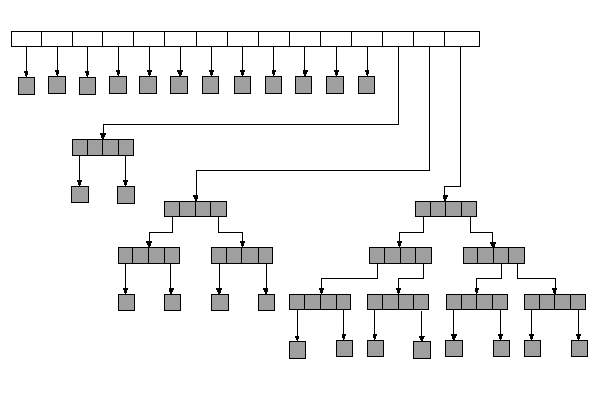
\includegraphics[width=120mm]{images/fig0419.png}
\caption{Adressering van datablokken in ext2}
\label{extAdressering}
\end{center}
\end{figure}

Het grote voordeel van deze structuur is dat de adresinformatie voor kleine bestanden volledig in het werkgeheugen
beschikbaar is. Met bestanden die maximaal 12 datablokken in beslag nemen kan dus erg snel gewerkt worden. Dat de
grootte van een bestand in ext2 beperkt is, volgt ook uit deze adresseringsstructuur. De maximale bestandsgrootte
in bytes wordt gegeven door:

\begin{displaymath}
S_{max} = \left[12 + \left(\frac{b}{4}\right) + \left(\frac{b}{4}\right)^{2} + \left(\frac{b}{4}\right)^{3}\right]b
\end{displaymath}

Hierin is $b$ de blokgrootte in bytes, en gaan we uit van adressen van 32 bits, dus 4 bytes per adres. Voor een
blokgrootte van 1 kB geeft dit een maximale grootte van 16GB.

\subsection{Vrije blokken en inodes}

In het superblok worden tabellen bijgehouden met de adressen van een aantal vrije datablokken en een aantal vrije
inodes. In deze tabellen is echter niet voldoende plaats om alle vrije elementen te bewaren.

Wanneer b.v. een bestand moet worden uitgebreid, wordt een adres van een vrij blok uit de tabel in het superblok
genomen. Bij het verwijderen van een bestand worden de adressen van de vrijgekomen blokken in de tabel ingeschreven.
Indien de tabel leeg is op het ogenblik dat een blok aan een file moet worden toegekend zal de tabel uit het eerste
blok in de gelinkte lijst naar het superblok worden gekopieerd. Het hierdoor vrijgekomen blok wordt aan het bestand
toegevoegd. Als de tabel helemaal gevuld is met adressen, en er wordt een blok vrijgegeven, dan wordt de tabel uit
het superblok naar het vrijgekomen blok gekopieerd, waarna dit als eerste blok in de gelinkte lijst wordt opgenomen.

Voor vrije inodes wordt een gelijkaardige methode gebruikt. In het superblok staat een tabel voor 100 nummers van
vrije inodes.  Wanneer een nieuw bestand vindt men hier het nummer van een beschikbare inode. Bij het verwijderen
van een bestand wordt het nummer van de hierdoor vrijgekomen inode aan de tabel toegevoegd.

Een belangrijk verschil met de vrije blokken is de mogelijkheid om een vrije inode te herkennen aan zijn inhoud. Het
veld voor het bestandstype staat namelijk op 0 als de inode niet in gebruik is. Hierdoor moeten niet alle nummers van
vrije inodes bijgehouden worden. Wanneer de tabel in het superblok leeg is, kan de kernel de i-list doorlopen en de
nummers van de 100 eerste vrije inodes in de tabel plaatsen.

Om het zoeken naar vrije inodes zo effici\"ent mogelijk te laten verlopen, wordt de positie van de laatst gevonden
vrije inode apart bijgehouden, om de volgende zoektocht vanop die positie te kunnen starten. Wanneer er een inode
vrijkomt door het verwijderen van een bestand zijn er dan 2 mogelijkheden. Als de positie van deze inode voor de
opgeslagen positie komt wordt de opgeslagen positie erdoor vervangen. Als de positie erna komt moet er niets gebeuren,
want dan wordt de nieuwe vrije inode zowiezo gevonden bij \'e\'en van de volgende zoektochten.

\subsection{Harde en zachte links}

Omdat de bestandsbeschrijving niet in de directory bewaard wordt, kan men op een eenvoudige en effici\"ente
manier eenzelfde bestand via verschillende paden aanspreken. Men laat in dit geval 2 bestanden verwijzen
naar eenzelfde inode, en dus ook naar hetzelfde bestand. Dit wordt een \emph{hard link} genoemd. Om een
acylische structuur te behouden is het niet toegelaten om hard links te cre\"eren naar directories
(zie eerder). Een hard link naar een bestand in een ander bestandssysteem kan ook niet. Voor
\emph{symbolische links} gelden deze beperkingen niet, maar in dit geval wordt verwezen naar een ander pad,
niet naar een inode.

Het gebruik van hard links vraagt ook om een speciale aanpak bij het verwijderen. De inode en de datablokken van
een bestand mogen pas vrijgegeven worden als er geen enkele link meer is. Daarom wordt in een inode een teller
met het aantal links bijgehouden (\verb|i_nlink|). Bij symbolic links is dit niet nodig. Wanneer het bestand
waarnaar een symbolic link verwijst verwijderd wordt, blijft de link bestaan. Zo'n link wordt een wees (orphan)
genoemd.

\subsection{Bijzonderheden}

Ext2 heeft enkele specifieke eigenschappen die we nog niet tegenkwamen in andere bestandssystemen. Zo wordt
het aantal inodes in de I-list bepaald bij het aanmaken van het bestandssysteem. Een vervelend
gevolg hiervan is dat het kan gebeuren dat je geen nieuw bestand kan aanmaken, hoewel er toch nog vrije
datablokken beschikbaar zijn. Een ext2 bestandssysteem heeft dus een maximum aantal bestanden. Standaard
wordt er \'e\'en inode aangemaakt voor iedere 4096 bytes beschikbare schijfruimte. Als de gemiddelde grootte
van je bestanden kleiner is dan 4kB, kan je dus met een tekort aan inodes te maken krijgen.

Bij het cre\"eren van het bestandssysteem wordt een deel (standaard 5\%) van de blokken gereserveerd voor
de beheerder van het syteem (root). Dit voorkomt dat een gebruiker of een gebruikersproces het volledige
bestandssysteem volschrijft, waardoor het besturingssysteem zou kunnen vastlopen.

Een laatste bijzonder bestandstype is de zogenaamde \emph{device file}. Deze bestanden bevatten geen data, maar
stellen een systeemapparaat voor. Zo kan men communiceren met een apparaat door te lezen en te schrijven van of
naar de bijhorende device file. Het toetsenbord zou je dan b.v. kunnen beschouwen als een oneindig alleen-lezen
tekstbestand. Ieder getypt karakter verschijnt in het bestand. Omdat lezen per blok voor een apparaat als een
toetsenbord niet erg effici\"ent zou zijn, wordt bij device files een onderscheid gemaakt tussen karakter- en
blokapparaten.
